\chapter{Modelos Ocultos De Markov}


En este capítulo, estudiaremos un tipo especial de proceso estocástico llamado modelo oculto de Markov (HMM). Empezaremos introduciendo estos modelos, para después seguir discutiendo sobre los problemas y algoritmos que conllevan. En adelante, utilizaremos la abreviatura HMM para referirnos a los modelos ocultos de Markov. 

Este capítulo se basa principalmente en \cite{Rabiner} y \cite{Russell}.

\section{Extensión a modelos ocultos de Markov}
Hasta ahora hemos considerado cadenas de Markov en las cuales cada estado es un evento observable (o material). Este modelo es demasiado restrictivo para aplicar a numerosos problemas en los cuales no podemos observar directamente los acontecimientos que nos interesan. Para estudiar estos problemas extendemos el concepto de modelo de Markov para incluir los casos en los que la observación es una función probabilística del estado. Como resultado, obtenemos un proceso estocástico conjunto formado por una cadena de Markov homogénea que no es observable (es decir, oculto) pero que produce una serie de consecuencias perceptibles mediante otro proceso estocástico. Es decir, tendremos una cadena $\{\mathcal{X}_t\}_{t=0}^{\infty}$ que representa los sucesos ocultos y un proceso $\{\mathcal{Y}_t\}_{t=0}^{\infty}$ que representa las consecuencias observadas de $\{\mathcal{X}_t\}$. 

Para aclarar esta idea, consideramos el siguiente ejemplo:

\begin{exampleth}\label{ejemplo_paraguas}
Un guardia de seguridad trabaja en una instalación subterránea, sin conexión con el exterior. Cada día, no puede saber si está lloviendo o no, pero por las mañanas ve llegar al director con o sin paraguas.

En este caso, $\mathcal{X}_t$ indica si llueve o no en el día $t$ e $\mathcal{Y}_t$ indica si el director lleva o no paraguas. Está claro que $\mathcal{Y}_t$ es consecuencia directa de $\mathcal{X}_t$ y asumiendo que la posibilidad de llover en un día determinado depende únicamente del tiempo del día anterior, tenemos que $\{\mathcal{X}_t\}$ es una cadena de Markov homogénea.

\end{exampleth}

Una representación común de la estructura de HMM es la siguiente:
\begin{figure}
\centering

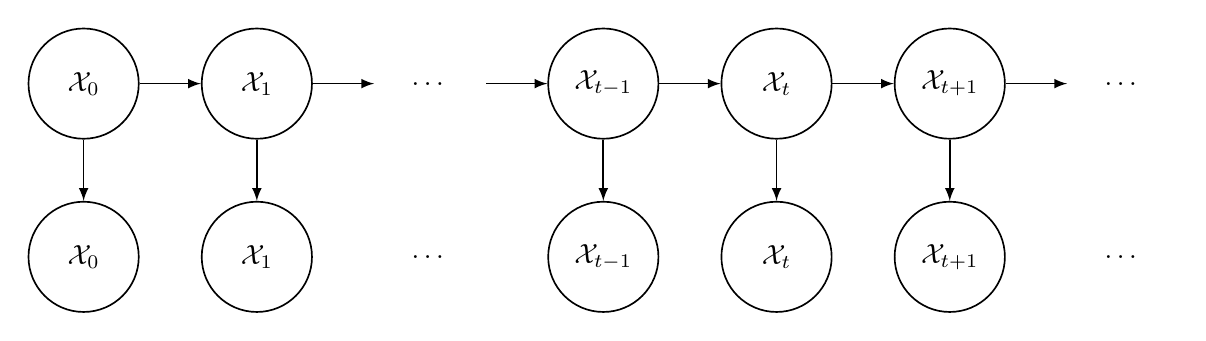
\begin{tikzpicture}[-latex ,auto , node distance =2.2 cm ,semithick,
main/.style = {draw, circle, minimum size=1.4cm}] 
    \node[main] (1) {$\mathcal{X}_0$}; 
    \node[main] (2) [right of=1] {$\mathcal{X}_1$};
    \node[main] (3) [right of=2, draw=none] {\dots};
    \node[main] (4) [right of=3] {$\mathcal{X}_{t-1}$};
    \node[main] (5) [right of=4] {$\mathcal{X}_{t}$};
    \node[main] (6) [right of=5] {$\mathcal{X}_{t+1}$};
    \node[main] (7) [right of=6, draw=none] {\dots};
    
    \node[main] (8) [below of=1] {$\mathcal{X}_0$}; 
    \node[main] (9) [right of=8] {$\mathcal{X}_1$};
    \node[main] (10) [right of=9, draw=none] {\dots};
    \node[main] (11) [right of=10] {$\mathcal{X}_{t-1}$};
    \node[main] (12) [right of=11] {$\mathcal{X}_{t}$};
    \node[main] (13) [right of=12] {$\mathcal{X}_{t+1}$};
    \node[main] (14) [right of=13, draw=none] {\dots};

    \draw (1) -- node[midway] {} (2);
    \draw (2) -- node[midway] {} (3);
    \draw (3) -- node[midway] {} (4);
    \draw (4) -- node[midway] {} (5);
    \draw (5) -- node[midway] {} (6);
    \draw (6) -- node[midway] {} (7);
    
    
    \draw (1) -- node[midway] {} (8);
    \draw (2) -- node[midway] {} (9);
    \draw (4) -- node[midway] {} (11);
    \draw (5) -- node[midway] {} (12);
    \draw (6) -- node[midway] {} (13);
    
\end{tikzpicture}
\caption{Estructura de un HMM}
\end{figure}

La representación anterior y el Ejemplo \ref{ejemplo_paraguas} nos da una idea de lo que es un HMM. Para concretarlo, damos la siguiente definición:

\begin{definition}
Sean $\{\mathcal{X}_t\}_{t=0}^{\infty}$ e $\{\mathcal{Y}_t\}_{t=0}^{\infty}$ procesos estocásticos que toman valores en conjuntos finitos $\mathbb{S}=\{s_1,\dots ,s_N\}$ y $\mathbb{V}=\{v_1,\dots ,v_M\}$ respectivamente. El proceso conjunto $\{\left(\mathcal{X}_t,\mathcal{Y}_t\right)\}$ es un modelo de Markov oculto si:
\begin{itemize}
    \item $\{\mathcal{X}_t\}$ es una cadena de Markov homogénea. 
    \item $P[\mathcal{Y}_t=y_t|\mathcal{X}_0=x_0,\dots,\mathcal{X}_t=x_t,\mathcal{Y}_0=y_0,\dots,\mathcal{Y}_{t-1}=y_{t-1}]=P[\mathcal{Y}_t=y_t|\mathcal{X}_t=x_t]$, es decir, la observación en el instante $t$ depende únicamente del estado que se encuentra en dicho momento.
\end{itemize}

\end{definition}

En distintas fuentes, en lugar de dar una definición explícita de HMM nombran los elementos que lo caracterizan. Puesto que son de enorme importancia, vamos a presentarlos a continuación. Un HMM se caracteriza por:
\begin{enumerate}
\item El conjunto de estados $\mathbb{S}=\{s_1,\dots ,s_N\}$ que, a pesar de no ser observables, suelen conllevar un significado físico del problema.
\item El conjunto de posibles observaciones $\mathbb{V}=\{v_1,\dots ,v_M\}$ que corresponden a las salidas materiales del sistema.
\item La matriz de transición $A$ asociada a $\{\mathcal{X}_t\}$ con:
\[a_{ij} = P[\mathcal{X}_{t+1}=s_j|\mathcal{X}_t=s_i]\]
\item Una matriz $B\in\left[0,1\right]^{N\times M}$ estocástica con:
\[b_{jk} = P[\mathcal{Y}_{t}=v_k|\mathcal{X}_t=s_j] \text{ para todo $t\geq0$}\]
Para reducir la confusión, en adelante utilizaremos la notación $b_{j}(k)$ para referirnos a estas probabilidades.
\item Una distribución inicial $\pi\in\Delta^{N-1}$ tal que:
\[P[\mathcal{X}_{0}=s_i]=\pi_i\]
\end{enumerate}

Es frecuente (véase \cite{Rabiner}) utilizar la notación:
\[\lambda=\left(A,B,\pi\right) \tag{2.\arabic{HMM}} \label{notacionHMM}\]
para representar un HMM.

\begin{section}{Los tres problemas básicos de los HMM}
A partir de los conceptos anteriores, podemos identificar 3 entidades: el modelo, la secuencia de observaciones o de salidas y la secuencia de estados. Existen 3 problemas básicos de interés que involucran a estas entidades \cite{Vidyasagar}:
\begin{enumerate}
\item Dado un HMM, ¿cuál es la probabilidad de observar una secuencia particular de salidas?
\item Dado un HMM y una secuencia de salidas, ¿cuál es la secuencia de estados más probable para generar dichas salidas?
\item Dada una secuencia de salidas y conociendo el espacio de estados, ¿cuál es el HMM que maximiza la probabilidad de observar dichas salidas?
\end{enumerate}

El \textbf{problema 1} es un problema de evaluación donde calculamos la probabilidad de observar una secuencia de salidas. También nos permite conocer si el modelo se ajusta a dicha secuencia. Esto puede ser útil, por ejemplo, si estamos considerando varios modelos posibles. En ese caso, la solución del \textbf{problema 1} nos permitiría elegir el modelo que más se ajuste a las observaciones.

En el Ejemplo \ref{ejemplo_paraguas}, un problema podría ser calcular la probabilidad de que el director lleve paraguas dos días seguidos y no en el tercero.

El \textbf{problema 2} es donde intentamos cubrir la parte oculta del modelo, es decir, a encontrar la secuencia \enquote{correcta} de estados. Está claro que en realidad no existe una secuencia \enquote{correcta}. Por ello, utilizaremos criterios de optimalidad para resolver este problema de la mejor manera posible. 

En el Ejemplo \ref{ejemplo_paraguas}, si se observa el paraguas en los dos primeros días y no en el tercero, parece lógico pensar que ha llovido en esos dos primeros días y no en el tercero. Veremos que es efectivamente así resolviendo este problema mediante el algoritmo de Viterbi.

En el \textbf{problema 3} pretendemos optimizar los parámetros del modelo dada una secuencia de salidas. La secuencia de observaciones usada para ajustar los parámetros se suele denominar secuencia de entrenamiento. El entrenamiento de HMM es importante, pues así podemos adaptar los parámetros a los datos percibidos. Y a partir de los resultados, podemos formular mejores modelos para describir fenómenos reales.

Como ejemplo , consideramos un problema de reconocimiento de voz, una de las aplicaciones más conocidas de HMM. Podemos utilizar las soluciones del \textbf{problema 3} para entrenar un HMM $\lambda_0$ (usando la notación \eqref{notacionHMM}) que reconoce la pronunciación del \enquote{no} y otro HMM $\lambda_1$ que reconoce la pronunciación del \enquote{sí}. Entonces, dada la pronunciación de una palabra desconocida, podemos usar la solución del \textbf{problema 1} para determinar si la palabra se asemeja más al \enquote{sí} o al \enquote{no}.  

En las siguientes subsecciones vamos a intentar solucionar estos problemas siguiendo principalmente la metodología descrita en \cite{Rabiner}. Notemos que, por ser $\{\mathcal{X}_t\}$ homogénea e $\mathcal{Y}_t$ depende únicamente del estado en el instante $t$, el instante en el que se comienza a observar las salidas es indiferente. Por lo tanto, podemos suponer siempre que las observaciones inician en el instante $t=0$.

\begin{subsection}{Solución al problema 1}
Queremos calcular la probabilidad de secuencia de observación concreta, $O=(O_0,O_1,\dots, O_r)$ conocido el modelo. La forma más directa de hacerlo es mediante enumeración de todas las posibles secuencias de estados de longitud $r+1$. Consideramos una de ellas:
\[Q=(q_0 , q_1 , \dots , q_r)\in\mathbb{S}^{r+1}\]
siendo $q_0$ el estado inicial. Para facilitar la escritura, introducimos la siguiente notación:
\[\mathcal{Y}_k^l:=(\mathcal{Y}_{k},\mathcal{Y}_{k+1},\dots,\mathcal{Y}_{l-1},\mathcal{Y}_{l})\]
Por lo tanto, la probabilidad de secuencia de observación dada la secuencia de estados $Q$ es:
\[P[\mathcal{Y}_0^r=O|\mathcal{X}_0^r=Q]=\prod_{t=0}^r P[\mathcal{Y}_{t}=O_t|\mathcal{X}_{t}=q_t]\]
donde aplicamos la independencia entre las observaciones. Por lo tanto:
\[P[\mathcal{Y}_0^r=O|\mathcal{X}_0^r=Q]=b_{q_0}(O_0)\cdot b_{q_1}(O_1)\cdots b_{q_r}(O_r)\]
Y la probabilidad de dicha secuencia de estados $Q$ se puede calcular como:
\[P[\mathcal{X}_0^r=Q]=\pi_{q_0}\cdot a_{q_0q_1}\cdot a_{q_1q_2}\cdots a_{q_{r-1}q_r} \]
Es claro que:
\[P[\mathcal{Y}_0^r=O,\mathcal{X}_0^r=Q]=P[\mathcal{Y}_0^r=O|\mathcal{X}_0^r=Q]\cdot P[\mathcal{X}_0^r=Q] \]
Y la probabilidad de $O$ se puede obtener sumando esta probabilidad mediante todas las posibles secuencias de estados:
\[P[\mathcal{Y}_0^r=O]=\sum_{Q\in\mathbb{S}^{r+1}}P[\mathcal{Y}_0^r=O|\mathcal{X}_0^r=Q]\cdot P[\mathcal{X}_0^r=Q]\]
\[=\sum_{(q_0 , q_1 , \dots , q_r)\in\mathbb{S}^{r+1}}\pi_{q_0}\cdot b_{q_0}(O_0)\cdot a_{q_0q_1}\cdot b_{q_1}(O_1)\cdots a_{q_{r-1}q_r}\cdot b_{q_r}(O_r)\]

Esta manera de calcular, involucra un orden de $2\cdot(r+1)\cdot N^{(r+1)}$ operaciones, puesto que existen $N^{(r+1)}$ posibles secuencias de estados, y para cada una de estas secuencias hay que realizar $2\cdot(r+1)$ cálculos. Esto hace imposible calcular esta probabilidad, pues incluso para un modelo de 5 estados, si se quiere calcular la probabilidad de una secuencia con 100 observaciones $(r=99)$ se necesitarían $2\cdot100\cdot5^{100}\approx10^{72}$ operaciones. Afortunadamente, existe una forma más eficiente de resolver \textbf{problema 1} y es mediante el conocido como \textbf{algoritmo de avance-retroceso}. 

\begin{definition}
Definimos la \textbf{variable de avance} $\alpha_t(i)$ como la probabilidad de observar la secuencia parcial $(O_0,O_1,\dots,O_t)$ y que el estado en el instante $t$ sea $s_i$:
\[ \alpha_t(i)=P[\mathcal{Y}_0^t=(O_0,\dots,O_t), \mathcal{X}_t=s_i]\]
\end{definition}
En el instante inicial $t=0$, para todo $i\in\{1,\dots,N\}$:
\[ \alpha_0(i)=P[\mathcal{Y}_0=O_0, \mathcal{X}_0=s_i]=P[\mathcal{Y}_0=O_0|\mathcal{X}_0=s_i]\cdot P[\mathcal{X}_0=s_i]=b_i(O_0)\cdot\pi_i\]
Suponiendo que conocemos las $\alpha_{t}(i)$ para todo $i$, podemos calcular fácilmente $\alpha_{t+1}(j)$, que es la probabilidad de observar $(O_0,O_1,\dots,O_{t+1})$ y $\mathcal{X}_{t+1}=s_j$. Puesto que queremos que $\mathcal{X}_{t+1}=s_j$, primero calculamos la probabilidad de mantener la misma secuencia parcial actualizado el estado, esto no es más que la suma de las variables de avance en $t$ multiplicados por las probabilidades de transición:
\[
\begin{aligned}
    P[\mathcal{Y}_0^r=O]&=\sum_{Q\in\mathbb{S}^{r+1}}P[\mathcal{Y}_0^r=O|\mathcal{X}_0^r=Q]\cdot P[\mathcal{X}_0^r=Q]\\
    &=\sum_{(q_0 , q_1 , \dots , q_r)\in\mathbb{S}^{r+1}}\pi_{q_0}\cdot b_{q_0}(O_0)\cdot a_{q_0q_1}\cdot b_{q_1}(O_1)\cdots a_{q_{r-1}q_r}\cdot b_{q_r}(O_r)
\end{aligned}    
\]
Dado que $\mathcal{Y}_{t+1}$ depende únicamente de $\mathcal{X}_{t+1}$, una vez conocida la suma anterior:
\[
\begin{aligned}
    \alpha_{t+1}(j)&=P[\mathcal{Y}_0^{t+1}=(O_0,\dots,O_t,O_{t+1}), \mathcal{X}_{t+1}=s_j]\\
    &=P[\mathcal{Y}_0^t=(O_0,\dots,O_t), \mathcal{X}_{t+1}=s_j]\cdot P[\mathcal{Y}_{t+1}=O_{t+1}|\mathcal{X}_{t+1}=s_j]\\
    &=\left(\sum_{i=1}^N\alpha_{t}(i)\cdot a_{ij}\right)\cdot b_j(O_{t+1})
\end{aligned}
\]
Luego podemos calcular las variables de avance de forma recursiva:
\begin{align*}
    &\alpha_{t+1}(j)=\left(\sum_{i=1}^N\alpha_{t}(i)\cdot a_{ij}\right)\cdot b_j(O_{t+1}), && 0\leq t\leq r-1\\ 
    & && 1\leq j\leq N \HMMadd \label{fowardRecursivo}
\end{align*}
Finalmente, notemos que:
\[
\HMMadd \label{fowardSecuencia}
P[\mathcal{Y}_0^r=O]=\sum_{i=1}^N P[\mathcal{Y}_0^r=O, \mathcal{X}_r=s_i]=\sum_{i=1}^N \alpha_r(i)\]
Si revisamos el cálculo de las variables de avance $\alpha_t(j)$, podemos ver que para cada estado se necesita $2N$ operaciones en una etapa $t>0$, puesto que hay $N$ estados, podemos concluir que el cálculo de todas las variables de avance requiere un orden de $2r N^2$ operaciones. Si $N=5$ y $r=99$, necesitaríamos alrededor de 5000 operaciones usando el algoritmo de avance, en comparación con $10^{72}$ operaciones que requiere en el cálculo directo. 

La parte de retroceso del algoritmo no es necesario para resolver \textbf{problema 1}, pero va a ser usada en la solución al \textbf{problema 3}, así que vamos a presentarla aquí. 

\begin{definition}
Definimos \textbf{la variable de retroceso} $\beta_t(i)$ como la probabilidad de observar la secuencia parcial $(O_{t+1},O_{t+1},\dots,O_{r})$ condicionada a que en el instante $t$, el estado sea $s_i$. Es decir:
\[\beta_t(i)=P[\mathcal{Y}_{t+1}^r=(O_{t+1},O_{t+2},\dots,O_{r})|\mathcal{X}_t=s_i]\]
\end{definition}

Puesto que la secuencia de salidas acaba en $O_r$, $\beta_r(i)$ no se puede determinar usando la definición anterior. En este caso, se define:
\[\beta_r(i)=1 \quad \forall i\in\{1,\dots,N\}\]
De forma similar a las variables de avance, podemos calcular $\beta_t(i)$ en base a $\beta_{t+1}(j)$. Puesto que conocemos éstos últimos, solo tenemos que preocuparnos por $O_{t+1}$. De nuevo, dado que $\mathcal{Y}_t$ depende únicamente de $\mathcal{X}_t$:
\[
\begin{aligned}
    &P[\mathcal{Y}_{t+1}^r=(O_{t+1},O_{t+2},\dots,O_{r})|\mathcal{X}_{t+1}=s_j]=\\
    &=P[\mathcal{Y}_{t+1}=O_{t+1}|\mathcal{X}_{t+1}=s_j]\cdot P[\mathcal{Y}_{t+2}^r=(O_{t+2},O_{t+3},\dots,O_{r})|\mathcal{X}_{t+1}=s_j]\\
    &=b_j(O_{t+1})\cdot\beta_{t+1}(j)
\end{aligned}
\]
Además, puesto que $\mathcal{X}_{t+1}$ depende de $\mathcal{X}_t$:
\[
\begin{aligned}
    \beta_t(i)&=P[\mathcal{Y}_{t+1}^r=(O_{t+1},O_{t+2},\dots,O_{r})|\mathcal{X}_t=s_i]\\
    &=\sum_{j=1}^N P[\mathcal{X}_{t+1}=s_j|\mathcal{X}_t=s_i]\cdot P[\mathcal{Y}_{t+1}^r=(O_{t+1},O_{t+2},\dots,O_{r})|\mathcal{X}_{t+1}=s_j]\\
    &=\sum_{j=1}^N a_{ij}\cdot b_j(O_{t+1})\cdot\beta_{t+1}(j)
\end{aligned}
\]

Luego también podemos calcular las variables de retroceso de forma recursiva:
\begin{align*}
    &\beta_t(i)=\sum_{j=1}^N a_{ij}\cdot b_j(O_{t+1})\cdot\beta_{t+1}(j), && 0\leq t\leq r-1\\ 
    & && 1\leq i\leq N \HMMadd \label{backwardRecursivo}
\end{align*}
Para cada estado, se necesita $3N-1$ operaciones en una etapa con $0\leq t\leq r-1$. Dado que existen $N$ estados, se requiere un orden de $3r N^2$ operaciones para calcular todas las variables de retroceso.

Veremos en los siguientes apartados, que las variables de avance y de retroceso serán usadas para resolver los \textbf{problemas 2 y 3}.
\end{subsection}

\begin{subsection}{Solución al problema 2}

A diferencia del \textbf{problema 1} donde podemos dar una solución exacta, existen varias maneras de resolver \textbf{problema 2}, donde queremos encontrar una secuencia de estados \enquote{óptima} dada una secuencia de observaciones. En primer lugar, debemos definir lo que es una secuencia de estados óptima. Existen varios criterios de optimalidad, una de ellas, se trata de escoger estados que son más probables individualmente. Con este criterio se pretende maximizar el número estimado de estados individuales correctos. Para implementar esta solución al \textbf{problema 2}, definimos la siguiente variable: 
\[\gamma_t(i)=P[\mathcal{X}_t=s_i|\mathcal{Y}_0^r=(O_0,O_1,\dots, O_r)]\]
que es la probabilidad de que el estado en el instante $t$ sea $s_i$ condicionado a observar la secuencia de salidas completa $O=(O_0,O_1,\dots, O_r)$.

\begin{proposition}
$\gamma_t(i)$ se puede expresar en función de las variables de avance y de retroceso:
\[\gamma_t(i)=\dfrac{\alpha_t(i)\cdot\beta_t(i)}{\sum\limits_{j=1}\limits^N \alpha_t(j)\cdot\beta_t(j)}\]
\end{proposition}
\begin{proofs*}
Por definiciones de las variables:
\[
\begin{aligned}
    \alpha_t(i)\cdot\beta_t(i)&=\\
    &=P[\mathcal{Y}_0^t=(O_0,\dots,O_t), \mathcal{X}_t=s_i]\cdot P[\mathcal{Y}_{t+1}^r=(O_{t+1},O_{t+2},\dots,O_{r})|\mathcal{X}_t=s_i]\\
    &=P[\mathcal{Y}_0^r=(O_0,O_1,\dots, O_r),\mathcal{X}_t=s_i]
\end{aligned}
\]
Por lo tanto:
\[
\begin{aligned}
    \dfrac{\alpha_t(i)\cdot\beta_t(i)}{\sum\limits_{j=1}\limits^N \alpha_t(j)\cdot\beta_t(j)}&=\dfrac{P[\mathcal{Y}_0^r=(O_0,O_1,\dots, O_r),\mathcal{X}_t=s_i]}{\sum\limits_{j=1}\limits^N P[\mathcal{Y}_0^r=(O_0,O_1,\dots, O_r),\mathcal{X}_t=s_j]}\\
    &=\dfrac{P[\mathcal{Y}_0^r=(O_0,O_1,\dots, O_r),\mathcal{X}_t=s_i]}{P[\mathcal{Y}_0^r=(O_0,O_1,\dots, O_r)}
\end{aligned}
\]
Aplicando la definición de probabilidad condicionada tenemos la igualdad del enunciado. \qed 
\end{proofs*}

Usando estas variables, podemos definir los estados más probables individualmente dada la secuencia de observaciones $O$:
\begin{definition}
Sea $O=(O_0,O_1,\dots,O_r)$, definimos el estado más probable individualmente en el instante $t$ como:
\[
\HMMadd \label{estadoProbableIndividualmente}
q_t=\argmax_{1\leq i\leq N}\{\gamma_t(i)\}=\{s_i\in\mathbb{S}\,|\,\forall s_j\in\mathbb{S}:\gamma_t(j)\leq\gamma_t(i)\}\]
\end{definition}

A pesar de que \eqref{estadoProbableIndividualmente} maximiza el número estimado de estados correctos, puede haber problemas con la secuencia de estados resultante. Por ejemplo, si existen estados inalcanzables desde una de ellas, la secuencia de estados \enquote{óptima} puede ser inválida. Esto se debe a que la solución proporcionada por \eqref{estadoProbableIndividualmente} sólo determina los estados más probables en cada instante, sin tener en cuenta la probabilidad de existencia de la secuencia resultante en ningún momento. 

Una posible solución a este problema es modificar el criterio. Se puede considerar secuencias de estados que maximizan el número estimado de parejas $(q_t,q_{t+1})$ o de tripleta $(q_t,q_{t+1},q_{t+2})$ de estados correctas. Estos criterios pueden ser razonables para ciertas aplicaciones concretas, pero el criterio más utilizado es el de encontrar la secuencia $Q=(q_0, q_1, \dots, q_r)$ que maximiza $P[\mathcal{X}_0^r=Q|\mathcal{Y}_0^r=O]$. Lo cual es equivalente a maximizar $P[\mathcal{X}_0^r=Q,\mathcal{Y}_0^r=O]$.

Una técnica formal para encontrar dicha secuencia $Q$ existe, se basa en métodos de programación dinámica y se llama algoritmo de Viterbi. En primer lugar definimos:
\[
\begin{aligned}
    \delta_t(i):&=\max_{(q_0,q_1\dots,q_{t-1})\in\mathbb{S}^t}P[\mathcal{X}_0^{t-1}=(q_0,q_1,\dots,q_{t-1}),\mathcal{X}_t=s_i,\mathcal{Y}_0^t=(O_0,\dots,O_t)]\\
    &=\max_{(q_0,q_1\dots,q_{t-1})\in\mathbb{S}^t}P[\mathcal{X}_0^{t}=(q_0,q_1,\dots,q_{t-1},s_i),\mathcal{Y}_0^t=(O_0,\dots,O_t)]
\end{aligned}
\]

En cada instante, $\delta_t(i)$ nos proporciona la probabilidad de la secuencia de estados más probable $(q_0,q_1,\dots,q_{t-1},q_t)$ de longitud $t+1$ con $q_t=s_i$, habiendo además observado $(O_0,\dots,O_t)$. 

En el instante inicial $t=0$, para todo $i\in\{1,\dots,N\}$:
\[
\begin{aligned}
    \delta_0(i)=P[\mathcal{X}_0=s_i,\mathcal{Y}_0=O_0]=P[\mathcal{X}_0=s_i]\cdot P[\mathcal{Y}_0=O_0|\mathcal{X}_0=s_i]=b_i(O_0)\cdot\pi_i
\end{aligned}
\]

Notemos que cada $\delta_t(i)$ con $t>0$ se puede calcular recursivamente en función de $\delta_{t-1}(j),1\leq j\leq N$. La idea principal de la recursión es que la secuencia más probable de estados hasta llegar a $\mathcal{X}_t=s_i$ está compuesta por la secuencia más probable $(q_0,q_1\dots,q_{t-1})$ con $q_{t-1}$ igual a un cierto estado $s_j$ y la transición de $s_j$ a $s_i$. Por lo tanto, tenemos que hallar las secuencias más probables hasta $t-1$ y ver desde cuál se obtiene la probabilidad máxima dando un paso más. Esta idea se puede ver con la siguiente gráfica:




\end{subsection}

\end{section}